\chapter{Constraint Propagation}

\section{Theoretical Foundations}

\subsection{Introduction to Constraint Programming}

Constraint programming is the study of computational systems based on constraints. The idea of constraint programming is to solve problems by stating constraints which must be satisfied by the solution.
\par
But, then, what is a constraint? It is simply a logical relation among several unknowns (or variables), each taking a value in a given domain. A constraint thus restricts the possible values that variables can take; it represents some partial information about the variables of interest.
Naturally, constraint programming problems have more than one constraint, and, to complicate things further, constraints are rarely independent.

\subsection{Constraint Satisfaction}

Currently there can be seen two branches of Constraint Programming research which arise from distinct bases and, thus, use different approaches to solve constraints. Constraint Satisfaction is one of the two branches, the other being Constraint Solving. For the purposes of this report, the focus will be on the former.

Constraint Programming divides in two branches, namely \textit{Constraint Satisfaction} and \textit{Constraint Solving}, which use different approaches to solve constraints. For the purposes of this report, the focus will be on the former, and specifically on \textit{Constraint Satisfaction Problems (CSPs)}

\paragraph{Constraint Satisfaction Problem (CSP)} A Constraint Satisfaction Problem (CSP) is defined mainly in three terms:

\begin{itemize}
    \item \textbf{Variables}: entities that can have multiple values assigned to them
    \item \textbf{Domains}: set of values that can be assigned to a variable
    \item \textbf{Constraints}: conditions that define what is considered a valid assignment to a variable; each constraint restricts the combination of values that a set of variables may take simultaneously
\end{itemize}

The solution of a CSP consists in assigning to each variable a value that satisfies all the constraints. Thus, the CSP is a combinatorial problem which can be solved by search. In the following sub-sections, basic systematic search methods, as well as techniques that improve on the latter, are discussed.

\subsection{Basic Systematic Search}

There are two main classes of systematic search algorithms.

\begin{itemize}
    \item algorithms that search the space of complete assignments, i.e., the assignments of all variables, till they find the complete assignment that satisfies all the constraints
    \item algorithms that extend a partial consistent assignment to a complete assignment that satisfies all the constraints.
\end{itemize}

\textbf{Backtracking (BT)} belongs to the latter class. In the BT method, variables are instantiated sequentially and as soon as all the variables relevant to a constraint are instantiated, the validity of the constraint is checked. If a partial assignment violates any of the constraints, backtracking is performed to the most recently instantiated variable that still has alternatives available. Clearly, whenever a partial assignment violates a constraint, backtracking is able to eliminate a portion of the search space, because the constraint-violating partial assignment will never be performed again.

\subsection{Consistency techniques}

The late detection of inconsistency is a main shortcoming of the BT paradigm. It is for this reason that various consistency techniques were introduced to overcome this disadvantage and preemptively prune the search space. Such techniques range from simple node-consistency and the very popular arc-consistency to full, but expensive path consistency.
For the purposes of this assignment, the most interesting techniques to delve into were the former two, that is, node consistency and arc consistency.

\paragraph{Node Consistency} The node representing a variable $X$ in a constraint graph is \textit{node consistent} if and only if for every value V in the current domain $D_X$ of $X$, each unary (meaning that it concerns only that variable) constraint on $X$ is satisfied.

\paragraph{Arc Consistency} An arc $(V_i, V_j)$ is \textit{arc consistent} if and only if, for every value $x$ in the current domain of $V_i$ which satisfies the constraints on $V_i$ there is some value $y$ in the domain of $V_j$ such that $V_i = x$ and $V_j = y$ is
permitted by the binary constraint between $V_i$ and $V_j$.

\subsection{Constraint Propagation}

By integrating systematic search algorithms with consistency techniques, it is possible to get more efficient constraint satisfaction algorithms. 
Therefore, a third possible schema was introduced that embeds a consistency algorithm inside a search algorithm. Such schemas are usually called look-ahead strategies and they are based on idea of reducing the search space through constraint propagation.
\par
Simple backtracking (BT) already performs some kind of consistency technique, which can be summarized as arc consistency checks between a newly instantiated (or updated) variable and already instantiated ones. As mentioned before, however, the inconsistency is detected late, at the last moment, highlighting the fact that there is a lot of room for search space reduction.
\par
\textbf{Forward checking} is the easiest way to achieve such a feat. The forward checking algorithm is based on the idea that future assignments cannot conflict with current ones. 
Arc consistency checks are performed between pairs of a not-yet instantiated variable and an instantiated one, as opposed to the simple BT algorithm that considers only pairs of already instantiated variables. Therefore, the invariance that \textit{for every un-instantiated variable there exists at least one value in its domain which is compatible with the values of instantiated variables} is maintained. Consequently, forward checking allows branches of the search tree that will lead to a failure to be pruned earlier than with backtracking.

\subsection{Ordering}

The efficiency of search algorithms which incrementally attempts to extend a partial solution depends considerably on the order in which variables are considered for instantiations. 
Usually, a static ordering of variables performs worse than a dynamic one, hence it is useful to consider greedy techniques such as choosing the variable with the smallest or biggest domain (most or less constrained) first.

\subsection{CSP Theory Applied to Sudoku}

As mentioned in the first chapter, Sudoku is a problem with clearly defined constraints, that is, for each variable, which is represented by a Sudoku cell, its value must not be assigned to other cells of the same row, column or box. It is therefore very intuitive to try to solve this problem by applying \textit{Forward Checking}: the domain of each cell, that is, the set of values available for assignment, must not contain values that are already assigned to cells of the same row, column or square. This way, future assignments are guaranteed to not violate any constraint, hence greatly reducing the search space.

\section{Software Implementation}

The core parts of the implementation are the main function, which implements the backtracking part of the solver, the way the forward checking and the domain updates are performed, and the chosen variable ordering technique. All of these aspects, as well as the fundamental data structures, are discussed in detail in the following sub-sections.

\subsection{Fundamental Data Structures}\label{cp_data_structs}

\subsubsection{CellCoordinates Class}

The \textit{CellCoordinates} class simply represents the pair of row and column indexes of some Sudoku cell. This class is widely used in the solver implementation, possibly paired with an integer value, to represent a full Sudoku cell.

\begin{figure}[h]
    \centering
    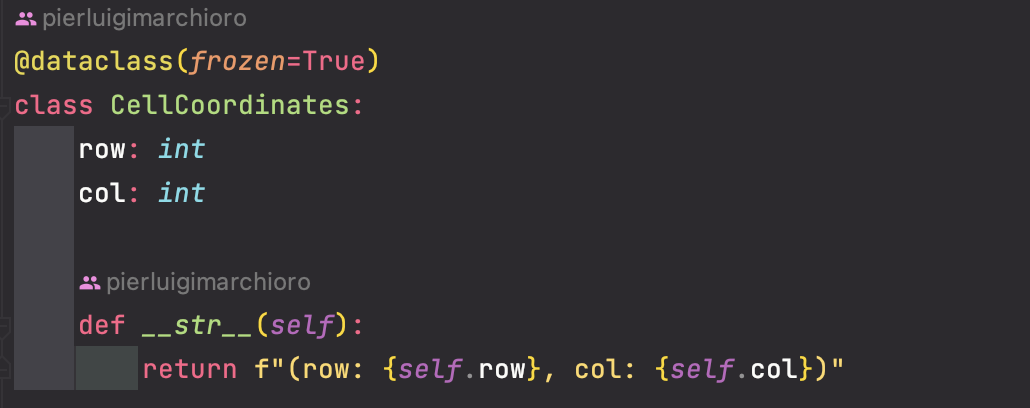
\includegraphics[scale=0.65]{assignment-1/images/cp/data-1-cell-coords.png}
    \caption{\textit{CellCoordinates} Class}
    \label{fig:data_1}
\end{figure}

\subsubsection{SudokuGrid Class}

The \textit{SudokuGrid} class provides a basic interface to access the cells of a Sudoku grid, that is, getters and setters for the whole grid, for single cells, or for whole rows, columns and squares.
Additionally, this class serves as super-type for some more specific implementations that provide functionality related to a specific solving technique, like the later discussed \textit{ConstraintPropagationSudokuGrid}.

\begin{figure}[h]
    \centering
    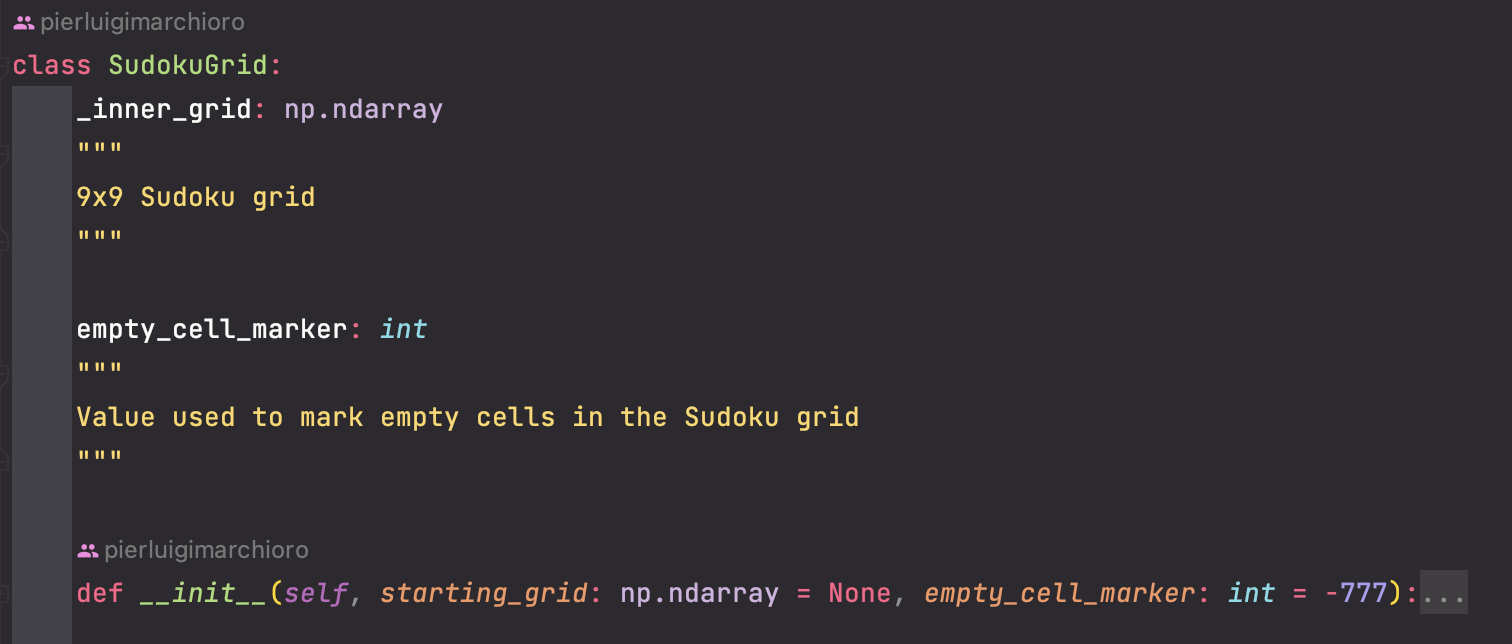
\includegraphics[scale=0.65]{assignment-1/images/cp/data-2_1-grid.png}
    \caption{\textit{SudokuGrid} Class (1) - The actual Sudoku grid is represented by a \textit{numpy} two-dimensional array}
    \label{fig:data_2_1}
\end{figure}

\begin{figure}[h]
    \centering
    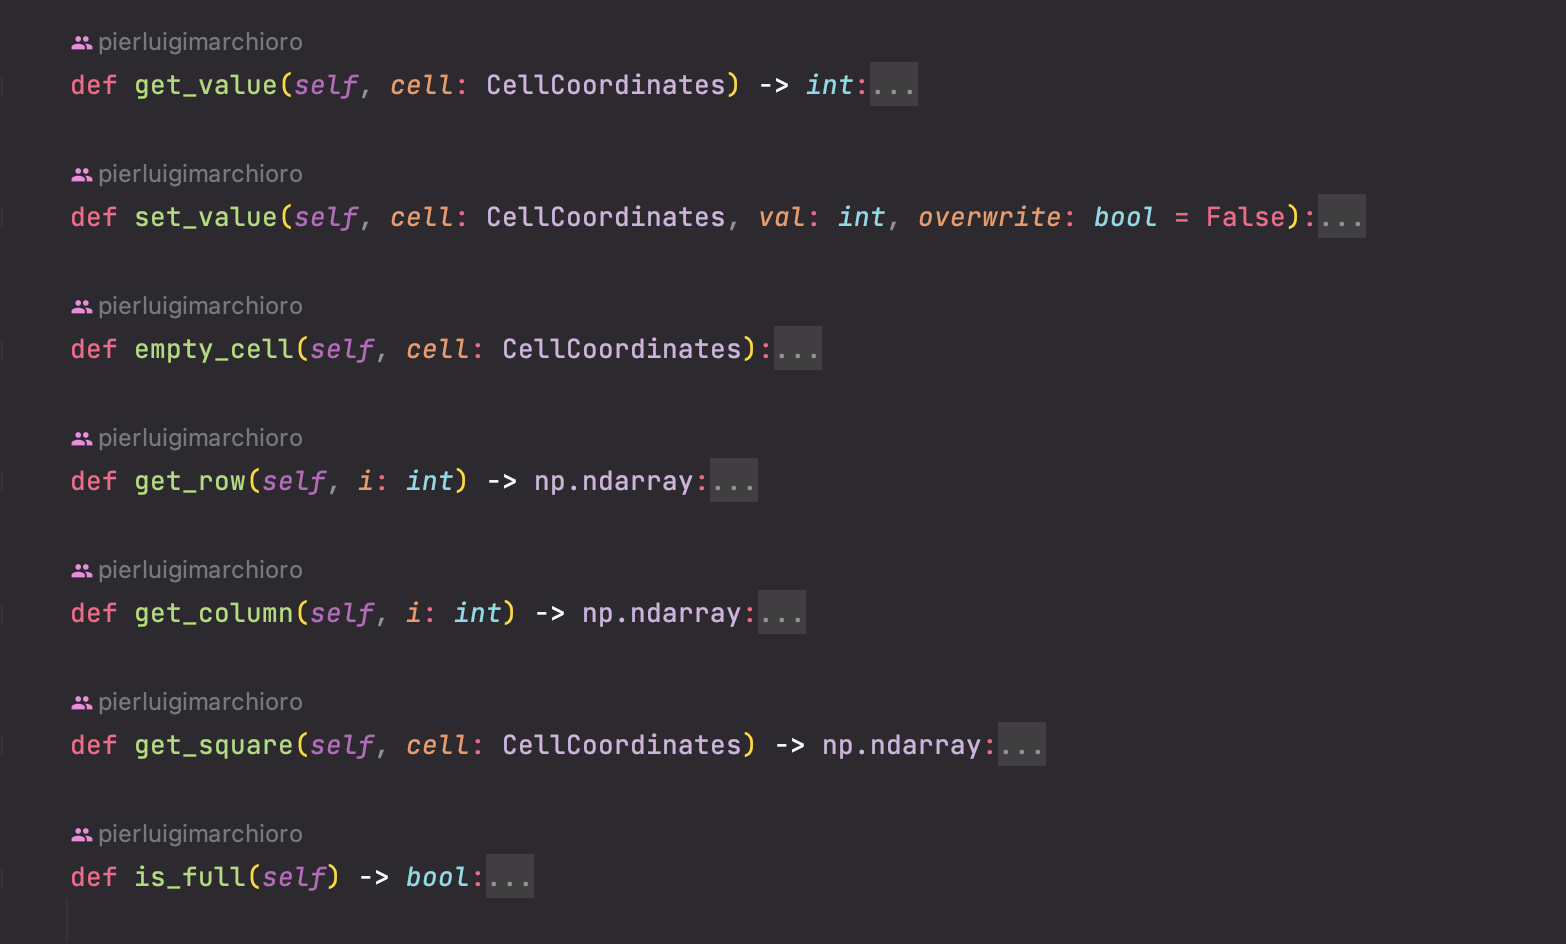
\includegraphics[scale=0.65]{assignment-1/images/cp/data-2_2-grid.png}
    \caption{\textit{SudokuGrid} Class (2)}
    \label{fig:data_2_2}
\end{figure}


\subsection{Main Function}

This part is the actual implementation of the Backtracking Sudoku-solving function. The main idea is of course to try to assign some value to some cell and then move on to the next; if a dead end is reached, the algorithm retraces back to the first cell with available assignments and tries again to move forward. 
As regards to this particular implementation, which makes use of \textit{Constraint Propagation}, the main steps of the algorithm are the following:

\begin{enumerate}
    \item \textbf{Choice of the Cell to Examine}: each iteration of the algorithm examines the most constrained cell at that point, that is, the cell whose domain is the smallest; this dynamic ordering of the variables was chosen because of the intuition that at least one value in each domain must be the correct one, so it's better to start from the cells with the fewest choices.

    \item \textbf{Backtracking}: the algorithm backtracks whenever a cell that has an empty domain is encountered, when every value in the domain of the current cell has been attempted, or when the grid is full but it isn't a valid solution.

    \item \textbf{Domain Updates}: during each move forward or backward of the algorithm, the domains of the cells affected by some new assignment are updated accordingly. Practically, this happens inside the \textit{grid.set\_value} and \textit{grid.empty\_cell} method calls, however such a process is discussed more in depth in the following sections.
\end{enumerate}

\begin{figure}[h]
    \centering
    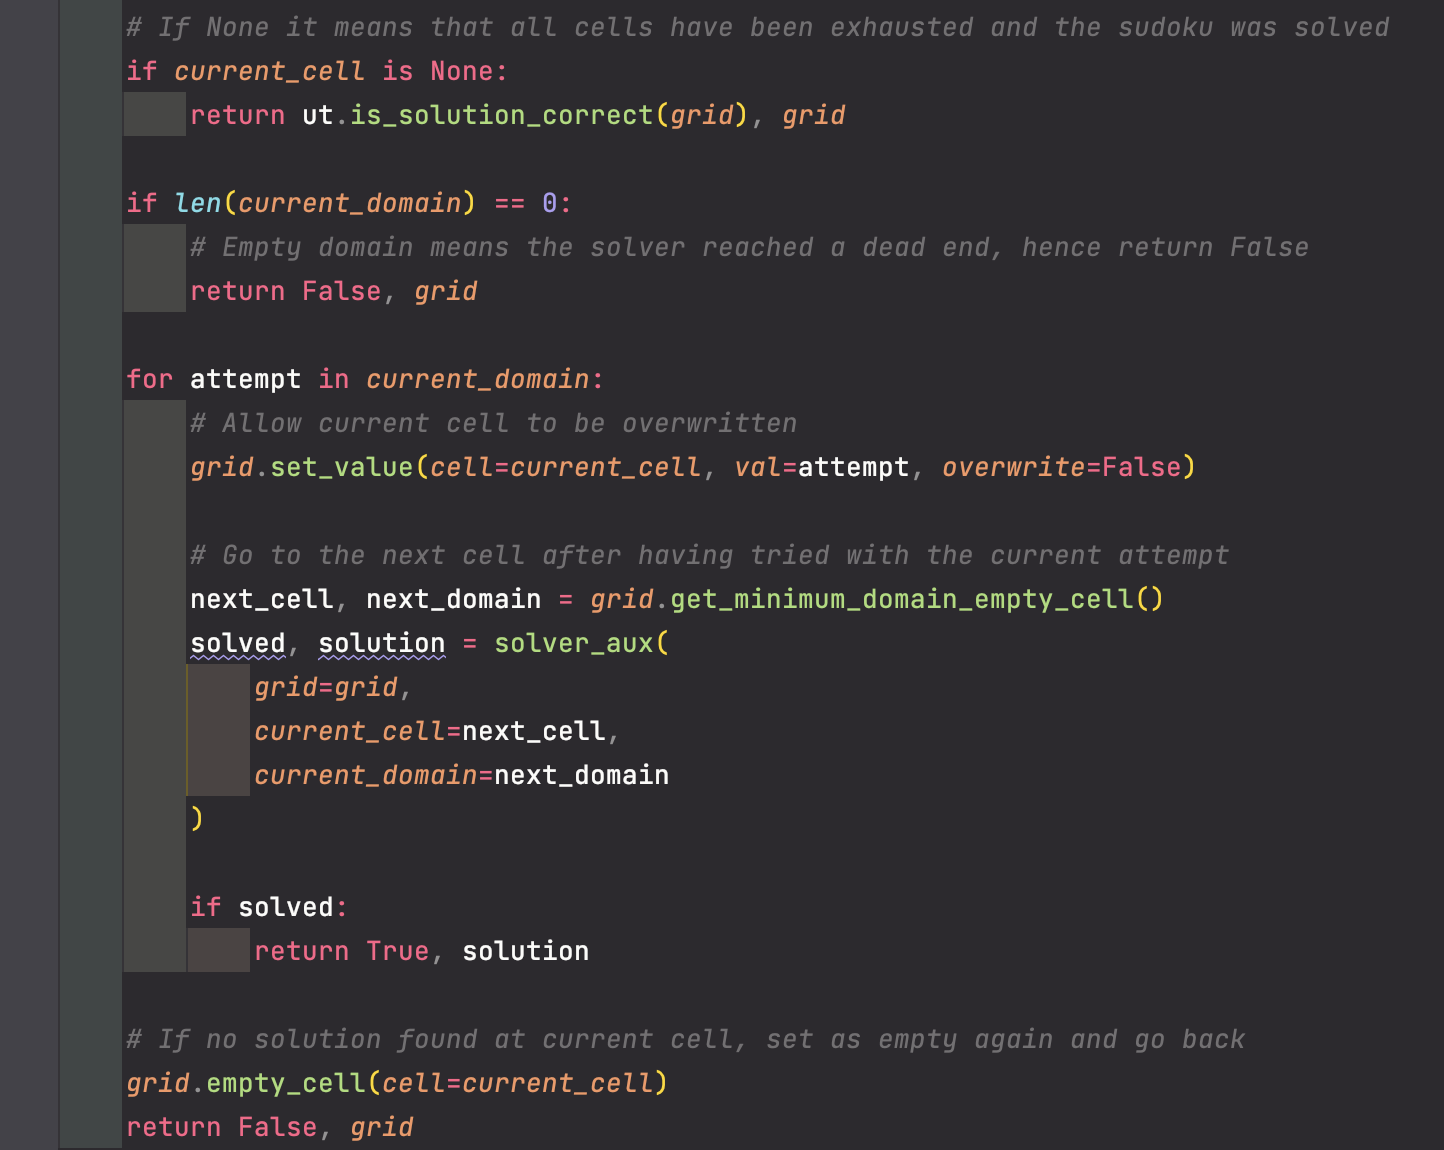
\includegraphics[scale=0.65]{assignment-1/images/cp/main.png}
    \caption{Main Body of the recursive BT algorithm - The domain of each empty cell is iterated through, starting from the most constrained cells}
    \label{fig:main_1}
\end{figure}

\subsection{Forward Checking and Domain Updates}

The actual \textit{Constraint Propagation} aspect of this solver is implemented through a form of \textit{Forward Checking}: after each assignment to some cell $C$, which can be both the action of setting a set to a new value and the action of emptying the cell, all the cells affected by it, that is, the cells that share the same row, column or box of $C$, have their domain updated to reflect only the values that can be assigned to them, in the future, without violating any constraint.
\par
More implementative details are discussed in the following sub-sections.

\subsubsection{Implementation of Cell Domains}

Cell domains were implemented as a dictionary that pairs each cell (coordinates) with its set of valid assignments, which are, of course, numbers from 1 to 9. Such a dictionary is a field of the \textit{ConstraintPropagationSudokuGrid} class, which, as the name says and as previously mentioned, implements constraint propagation functionality.

\begin{figure}[h]
    \centering
    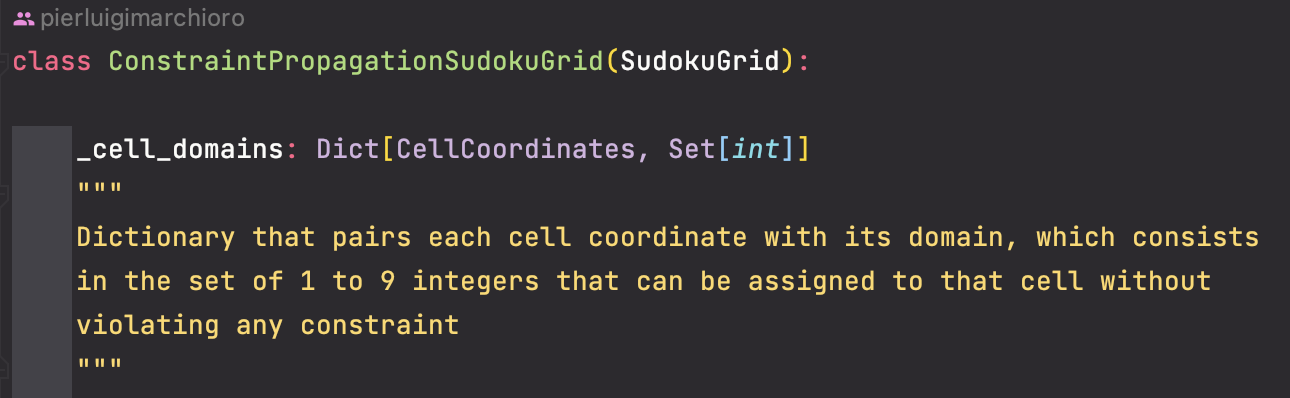
\includegraphics[scale=0.65]{assignment-1/images/cp/domains-1.png}
    \caption{Implementation of cell domains - Python dictionary that pairs each cell (coordinates) with its set of valid assignments}
    \label{fig:domain_1}
\end{figure}

\subsubsection{Implementation of Domain Updates on New Assignments}

The basic operations to update the domains of cells affected by new assignments are, in fact, the calculation of the domain of a single cell, and the calculation of the set of cells affected by some assignment.

\paragraph{Cell Domain Calculation} The domain of a cell $C$ is defined as the set of values that can be assigned to it without violating any constraint, which means that such values must necessarily not occur in the row, column and box that $C$ belongs to. Such a set is obtained as the intersection of the sets of values not contained in such collections of cells.

\begin{figure}[h]
    \centering
    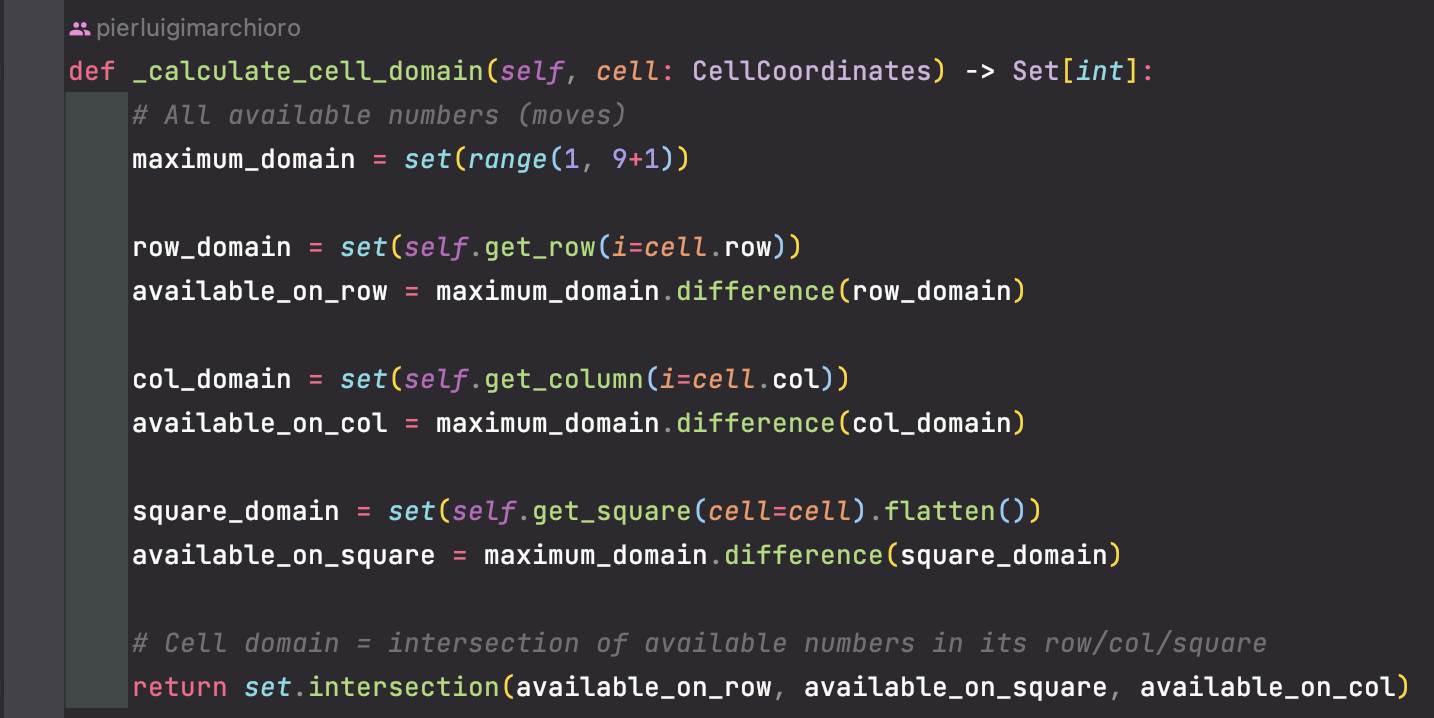
\includegraphics[scale=0.65]{assignment-1/images/cp/domains-2-calc-cell-dom.png}
    \caption{Calculation of the domain of a single cell}
    \label{fig:domain_2}
\end{figure}

\paragraph{Affected Cells Calculation} The set of cells affected by a new assignment to some cell $C$ is simply calculated as the set of coordinates belonging to the cells that share the same row, column or box as $C$.

\begin{figure}[h]
    \centering
    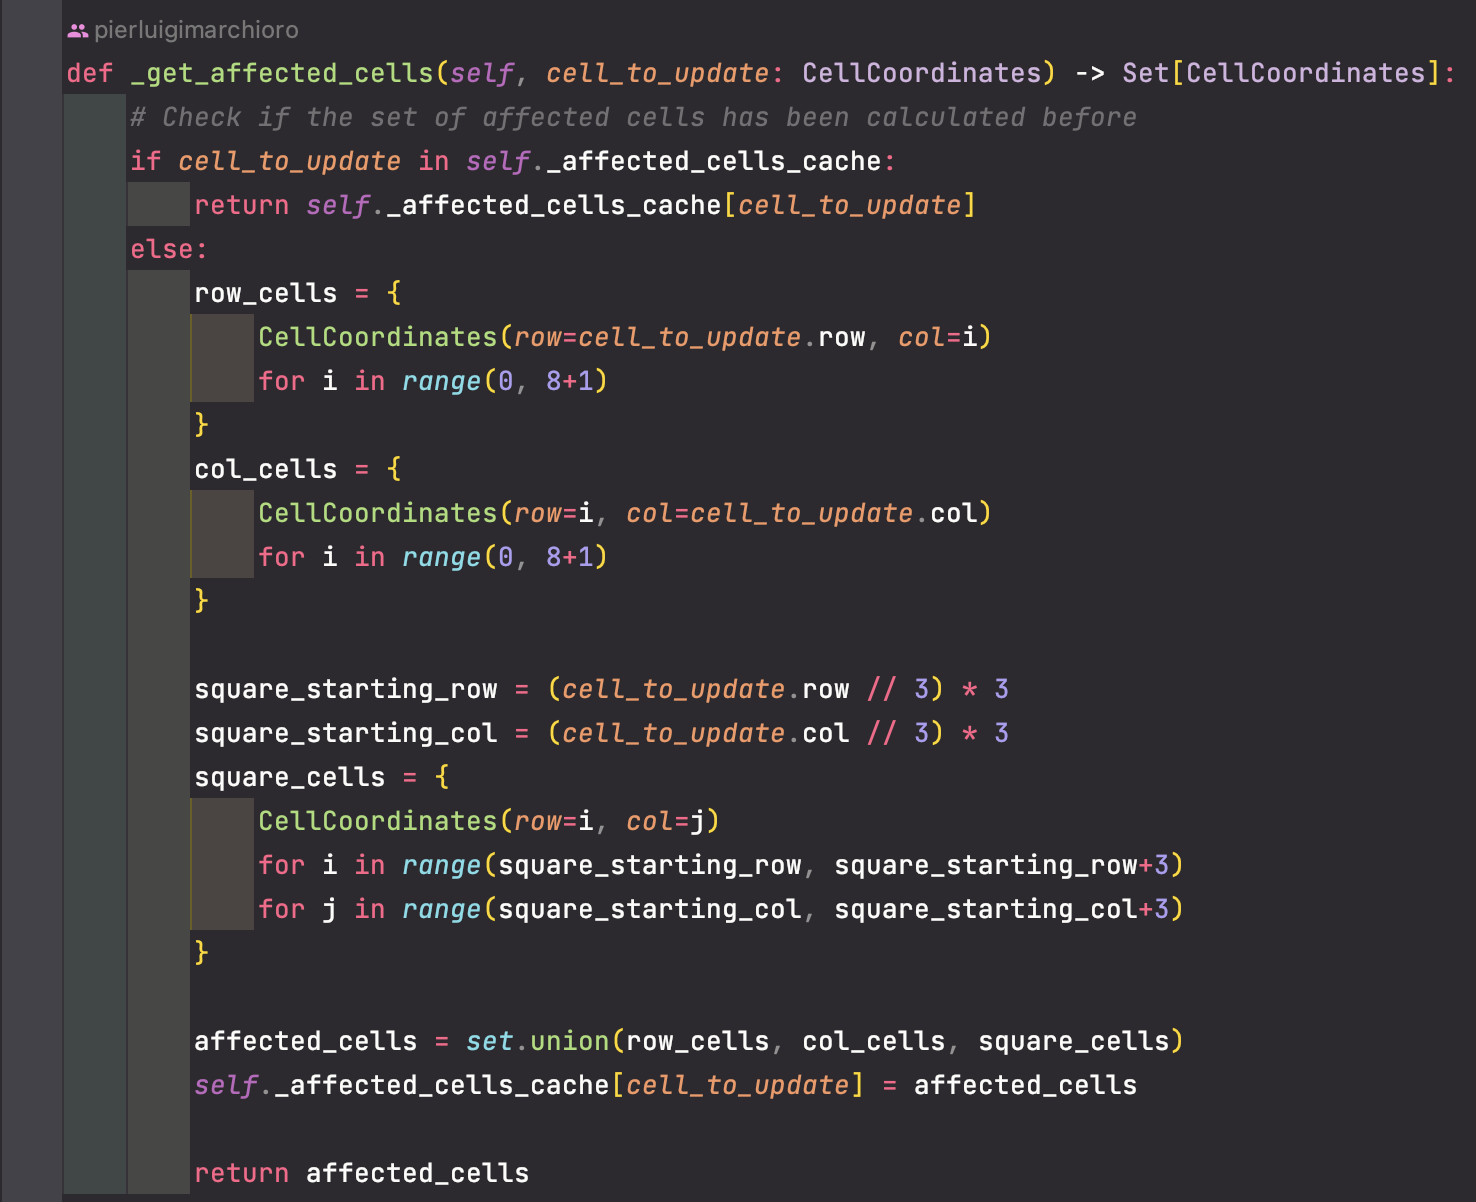
\includegraphics[scale=0.65]{assignment-1/images/cp/domains-3-calc-affected-doms.png}
    \caption{Calculation of the set of cells affected by the assignment of a new value to some cell $C$ - It is noted that the results of each call are cached, because the set of affected cells of $C$ never changes}
    \label{fig:domain_3}
\end{figure}

\par
As regards to the actual updates to the domains, they are performed in different manners, depending on the type of the new assignment.

\paragraph{Emptying a Cell} In such a case, the domains of all the affected cells are recalculated entirely, because it is not certain that all of the former would expand after removing one number from the grid; if that was the case, then it would've been enough to just add the removed value back to them.

\paragraph{Filling a Cell} In such a case, the new value is simply removed, if present, from the domains of the affected cells. This is a simple condition to check, and it is far more efficient than recalculating domains in their entirety.

\begin{figure}[h]
    \centering
    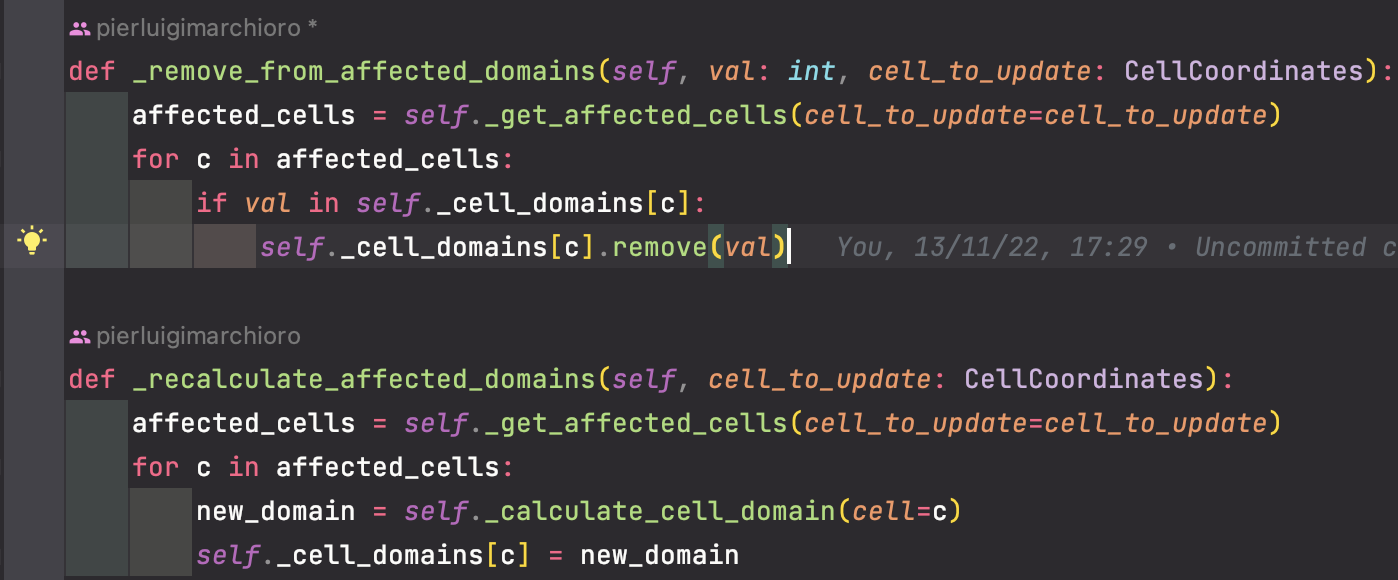
\includegraphics[scale=0.65]{assignment-1/images/cp/domains-4-recalc-remove-doms.png}
    \caption{Update of the domains of the cells affected by a new assignment}
    \label{fig:domain_4}
\end{figure}

\subsection{Ordering Technique}

As discussed before, the algorithm leverages a dynamic ordering of the variables, that is, the Sudoku cells, which is based on the dimension of their domains; specifically, the most constrained empty cell is chosen first. Below is the implementation of this ordering mechanism.

\begin{figure}[h]
    \centering
    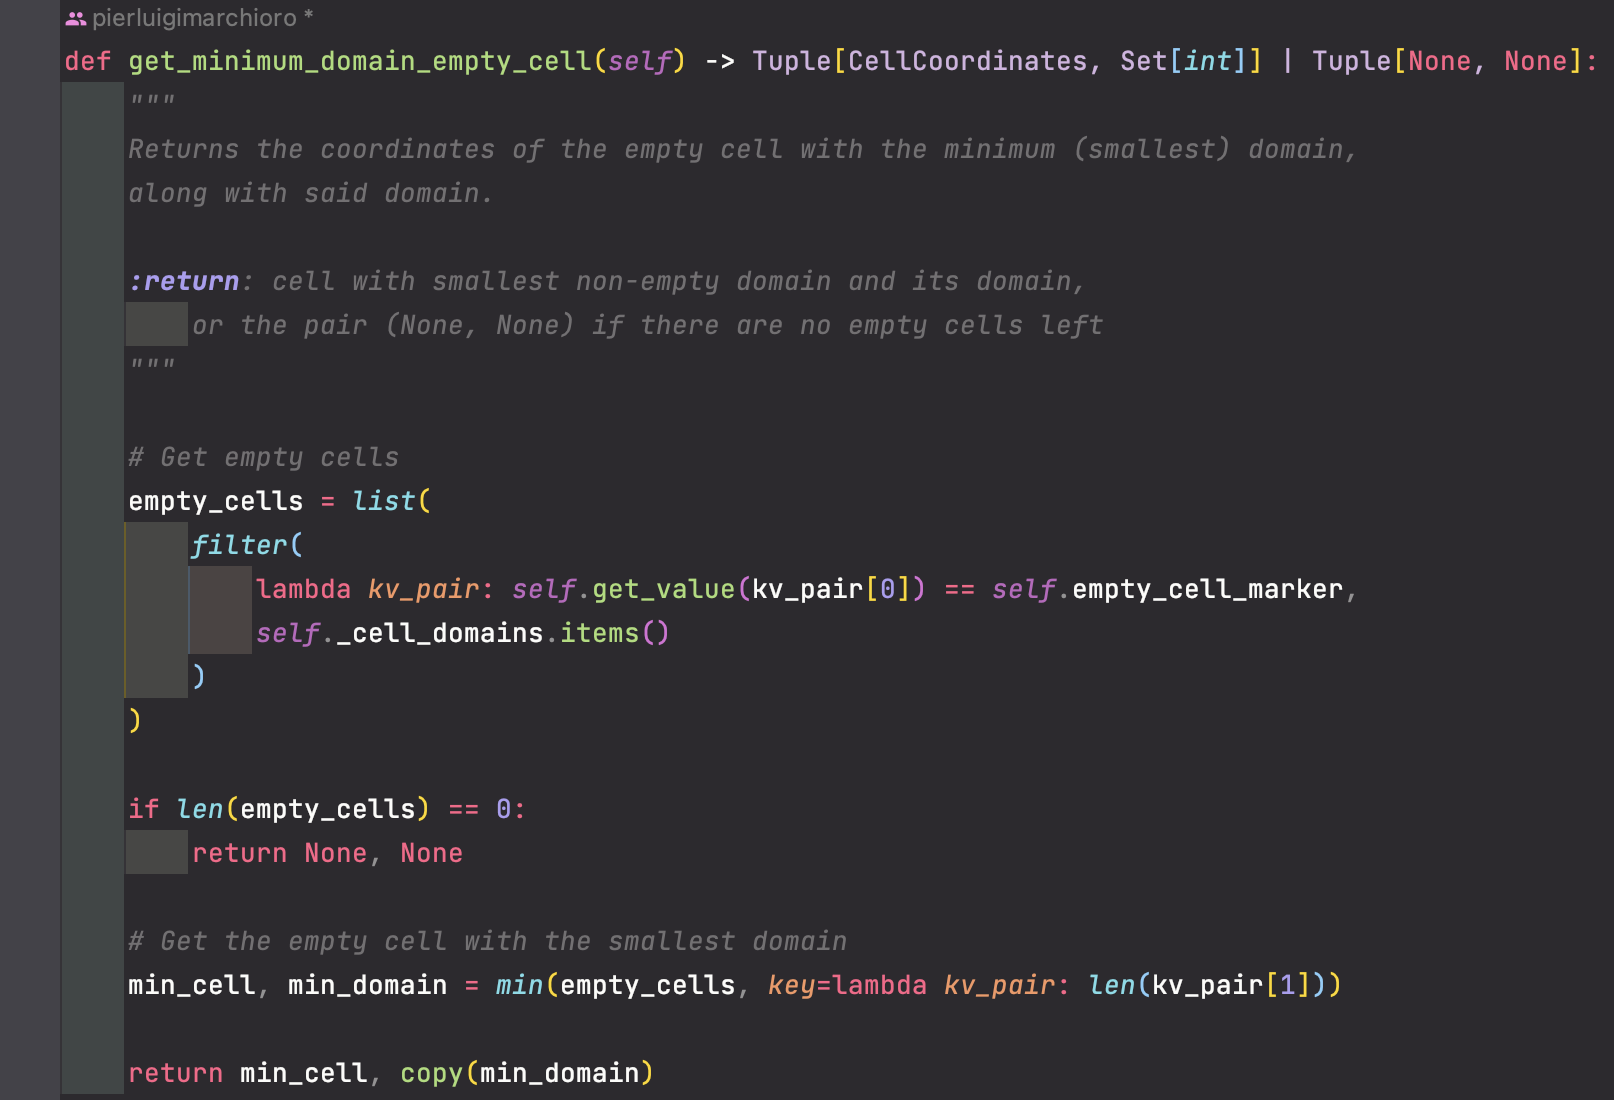
\includegraphics[scale=0.5]{assignment-1/images/cp/ordering-1.png}
    \caption{Implementation of dynamic ordering - the most constrained cell is chosen first}
    \label{fig:ordering_1}
\end{figure}



